

\textbf{1. Exact expression}.
Consider the Coulomb interaction in second quantization between electrons:
\begin{equation*}
	\blue{\hat{V}} = \frac{1}{2 \mathcal{V}} \sum_{\sigma \sigma'} \sum_{k k' q} V(q) 
	\blue{c\D_{k + q,\sigma} c\D_{k'-q,\sigma'} c_{k', \sigma'} c_{k, \sigma}},
\end{equation*}
$\mathcal{V}$ is the volume. Taking into account only scattering processes that involve two
particles, we could derive an expression for the inverse life time $1/ \tau_k$ of the state\footnote{
	Here and further $\overset{\mathrm{n}}{=}$ means that we ignore normalization factor, that appears in $\mathcal{N}_{i,f}$.
} $\ket{i} = \ket{k_1, \sigma_1} \overset{\mathrm{n}}{=}  c\D_{k_1, \sigma_1} \ket{\Omega}$, where $\ket{\Omega}$ denotes the state, where all states below Fermi surface are occupied. 


With Fermi's Golden Rule (fig. \ref{fig:absd}b)
\begin{equation*}
	\frac{1}{\tau_{k_1}} = 2 \pi \sum_{f} |\bk{f}[\blue{\hat{V}}]{k, \sigma}|^2 \delta(\varepsilon_i - \varepsilon_f),
	\hspace{10 mm}
	\ket{f} \overset{\mathrm{n}}{=}  c\D_{k_1-Q,\sigma_1} c\D_{k_2+Q,\sigma_2} c_{k_2,\sigma_2} \ket{\Omega}. 
\end{equation*}
Thus life time could be expressed from the matrix elements
\begin{equation*}
% \bk{k_1, \sigma_1} [\blue{\hat{V}}]{k_1-Q,\sigma_1; k_2+Q,\sigma_2; \cancel{k_2, \sigma_2}} 
\bk{i} [\blue{\hat{V}}]{f} 
= 
\frac{1}{2 \mathcal{V}} \sum_{\sigma \sigma'} \sum_{k' q} \mathcal{N}_{i,f} V(q) 
	\bk{\Omega}[
		c_{k_1, \sigma_1}  
		\blue{c\D_{k + q,\sigma} c\D_{k'-q,\sigma'} c_{k', \sigma'} c_{k, \sigma}}   
		c\D_{k_1-Q,\sigma_1} c\D_{k_2+Q,\sigma_2} c_{k_2,\sigma_2}
	]{\Omega},
\end{equation*}
with normalizing factor 
\begin{equation*}
	\mathcal{N}_{i,f} = \left(
		(1- n_{k_1, \sigma_1})(1- n_{k_1-Q, \sigma_1}) (n_{k_2, \sigma_2})(1- n_{k_2+Q, \sigma_2})
	\right)^{-1/2},
\end{equation*}
since $\langle c\D c\rangle = n$ and $\langle c c\D\rangle = 1-n$.


\begin{figure}[h]
    \centering
    \vspace{-10mm}
    \addletter{80}{a} \hspace{5 mm} 
    \begin{tikzpicture}
	\begin{feynman}[large]
		\vertex (i1);
		\vertex [below right=of i1] (a);
		\vertex [below left=of a] (i2);
		\vertex [right=of a] (b);
		\vertex [above right=of b] (f1);
		\vertex [below right=of b] (f2);
		\diagram* {
		(i1) -- [fermion, edge label=\(k\,\sigma\)] (a) -- [fermion, edge label=\(k+q\,\sigma\)] (i2),
		(f1) -- [fermion, edge label'=\(k'\,\sigma'\)] (b) -- [fermion, edge label=\(k'-q\,\sigma'\)] (f2),
		(a) -- [boson] (b),
		};
	\end{feynman}
	\end{tikzpicture}
	\hspace{10 mm} 
	\addletter{80}{b}
    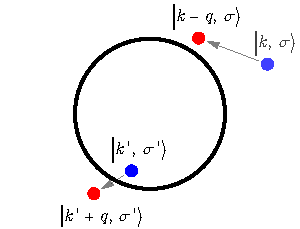
\includegraphics{imgs/FSe.pdf}
    \caption{Scattering process}
    \label{fig:absd}
\end{figure}

% Осталось подружить друг с другом состояния.
To calculate this matrix element we need just to decide how to distribute $\ket{k_1, \sigma_1}$, $\ket{k_2, \sigma_2}$, $\ket{k_1-Q, \sigma_1}$, $\ket{k_2+Q, \sigma_2}$ over the $\ket{k, \sigma}$, $\ket{k', \sigma'}$, $\ket{k'-q, \sigma'}$, $\ket{k+q,\sigma}$ (fig. \ref{fig:absd}a). There are only two different ways to do this (\red{sign} could be found as in the Wick's theorem):
\begin{align*}
	% \bk{k_1, \sigma_1} [\blue{\hat{V}}]{k_1-Q,\sigma_1; k_2+Q,\sigma_2; \cancel{k_2, \sigma_2}} = 
	\bk{i}[\hat{V}]{f}_1 
	&= 
	\frac{\mathcal{N}_{i,f}}{2\mathcal{V}} \sum_{k,k',q} \sum_{\sigma_1,\sigma_2} V(q)   \delta_{\sigma_1, \sigma} \delta_{\sigma_2, \sigma'} \delta(k_1-k-q)  \delta(Q-q) (1-n_{k_1}) n_{k_2} (1-n_{k_1-Q}) (1-n_{k_2+Q})
	\\ &= 
	\frac{\mathcal{N}_{i,f}}{2\mathcal{V}} V(Q) (1-n_{k_1, \sigma_1}) n_{k_2,\sigma_2} (1-n_{k_2+Q,\sigma_2})(1-n_{k_1-Q,\sigma_1})
	,
\end{align*}
and
\begin{align*}
	\bk{i}[\hat{V}]{f}_2 = \ldots
	% \red{-}\mathcal{N}_{i,f}\sum_{k,k',q} \sum_{\sigma_1,\sigma_2}V(q) \delta_{\sigma_1, \sigma} \delta_{\sigma_2, \sigma'} \delta(k_1-k-q)  \delta(k_2-k'+q) \delta(Q-q) (1-n_{k_1}) n_{k_2} (1-n_{k_1-Q}) (1-n_{k_2+Q}) 
	= \red{-} \frac{\mathcal{N}_{i,f}}{2\mathcal{V}} V(k_1-k_2-Q) \delta_{\sigma_1, \sigma_2} 
	(1-n_{k_1,\sigma_1} )
	n_{k_2,\sigma_2}
	(1-n_{k_2+Q,\sigma_2})
	(1-n_{k_1-Q,\sigma_1})
	.
\end{align*}
Due to symmetry, each term will appear twice, which means
\begin{equation*}
	\bk{i}[\hat{V}]{f} = \frac{\mathcal{N}_{i,f}}{\mathcal{V}} V(Q) (1-\delta_{\sigma_1,\sigma_2}) (1- n_{k_1, \sigma_1})(1- n_{k_1-Q, \sigma_1}) (n_{k_2, \sigma_2})(1- n_{k_2+Q, \sigma_2}) = \frac{1-\delta_{\sigma_1,\sigma_2}}{\mathcal{V} \mathcal{N}_{i,f}} V(Q).
\end{equation*}
As expected, we found that only particles with different spins are scattered.


Let's move on to integration
\begin{equation*}
	\frac{1}{\tau_{k_1}} 
	= 
	2 \pi \sum_{f} |\bk{f}[\blue{\hat{V}}]{k, \sigma}|^2 \delta(\varepsilon_i - \varepsilon_f) 
	= 
	\frac{2\pi}{\mathcal{V}^2} \int \frac{d^3 k_2\ d^3 Q}{(2\pi)^6} |V(Q)|^2 \mathcal{N}_{i,f}^{-2}
	\delta(\varepsilon_i - \varepsilon_f) \sum_{\sigma_2} (1-\delta_{\sigma_1,\sigma_2}),
\end{equation*}
with $\varepsilon_i - \varepsilon_f = \varepsilon_{k_1} - \varepsilon_{k_1-Q} - \varepsilon_{k_2+Q} + \varepsilon_{k_2}$.


% kkhoruzhii
% 256494936Fermi!




\textbf{2. Approximate calculation}. 
By anticipating the result for the screening of the Coulomb interaction, we can
assume that  $V(Q) \approx V(0) = \const$. It is convenient to use  (with $\xi = \varepsilon - \varepsilon_F$ and $d \vc{k} = d \cos \theta \, d \varphi$)
\begin{equation*}
	\int \frac{d^3 k}{(2\pi)^3} 
	= \int \frac{d \vc{k}}{4\pi} \int d\xi \, N(\xi)  
	=  N(0)\int \frac{d \vc{k}}{4\pi} \int \d \xi
	.
\end{equation*}
We consider system at $T=0$:
\begin{equation*}
	(1- n_{k_1, \sigma_1})(1- n_{k_1-Q, \sigma_1}) (n_{k_2, \sigma_2})(1- n_{k_2+Q, \sigma_2}) = \theta(\xi_{k_1}) \theta(- \xi_{k_2}) \theta(\xi_{k_1-Q}) \theta(\xi_{k_2+Q}).
\end{equation*}
Substituting this into the expression for the lifetime, we find
\begin{equation*}
	\frac{1}{\tau_{k_1}} \approx \frac{2\pi}{\mathcal{V}^2} |N(0)|^2 V(0)^2
	\int d \xi_{k_2} 
	\int \frac{d \vc{k}_{k_2}}{4\pi} 
	\int d \xi_{Q} 
	\int \frac{d \vc{k}_{Q}}{4\pi} 
	\theta(\xi_{k_1}) \theta(- \xi_{k_2}) \theta(\xi_{k_1-Q}) \theta(\xi_{k_2+Q})
	\delta( \varepsilon_{k_1} - \varepsilon_{k_1-Q} - \varepsilon_{k_2+Q} + \varepsilon_{k_2}).
\end{equation*}
Let's define $k_f = k_1 - Q$. As in the fig. \ref{fig:absd}b we take $\xi_{k_1} > 0$ and $\xi_{k_2+Q} > 0$
 % and $\xi_{k_f} < `$
\begin{equation*}
	\delta( \varepsilon_{k_1} - \varepsilon_{k_f} - \varepsilon_{k_1+k_2-k_f} + \varepsilon_{k_2}) = \frac{1}{2 \varepsilon_F} \delta\left(
		1 + \tilde{\vc{k}}_1 \cdot \tilde{\vc{k}}_2 - \tilde{\vc{k}}_1 \cdot \tilde{\vc{k}}_f - \tilde{\vc{k}}_2 \cdot \tilde{\vc{k}}_f
	\right),
\end{equation*}
with $\tilde{\vc{k}} = \vc{k} / k$. Rewriting the integral for the last time
\begin{equation*}
	\frac{1}{\tau_{k_1}} \approx  \frac{2\pi}{\mathcal{V}^2} |N(0)|^2 V(0)^2 \int_{-\xi_{k_1}}^{0} d \xi_{k_2} \int_{0}^{\xi_{k_1}-\xi_{k_2}} d \xi_{k_f} 
	\int \frac{d \vc{k}_{k_2}}{4\pi} \int \frac{d \vc{k}_{Q}}{4\pi} 
	\frac{1}{2 \varepsilon_F} \delta\left(
		1 + \tilde{\vc{k}}_1 \cdot \tilde{\vc{k}}_2 - \tilde{\vc{k}}_1 \cdot \tilde{\vc{k}}_f - \tilde{\vc{k}}_2 \cdot \tilde{\vc{k}}_f
	\right),
\end{equation*}
so finally
\begin{equation*}
	\frac{1}{\tau_{k_1}} \propto (\varepsilon_{k_1}-\varepsilon_F)^2.
\end{equation*}